\section{Conditional depth and placement distributions}
\label{sec:conditional-depth-calibration}

The preceding dimension profile could not exclude the 0.65\,m prior under its
declared heuristic band. We therefore evaluate a distribution over unresolved
depth, with its loss scale selected on separate procedural geometries. This
revision retains the observed-instance domain, qualified outside orientation,
width, box/leg height and absolute-layer construction of the preceding
outer-orientation/layer model. Uncertainty over those quantities, missing
parts, camera pose and instance association is not represented by the depth
distribution.

\paragraph{Joint geometry and structure update.}
Let $[u_{\min},u_{\max}]$ be the acquired support interval on the estimated
local depth axis, with span $s=u_{\max}-u_{\min}$. A continuous uniform prior
on $d\in[0.2,1.4]$\,m is conditioned on this observed span. Its quadrature
nodes have 0.1\,m spacing and include the acquired lower boundary; masses are
clipped Voronoi-cell lengths, rather than equal masses at irregular nodes.
A credible observed endpoint fixes that endpoint. Without either endpoint,
the lower coordinate is
\begin{equation}
 \ell_k=u_{\min}-a_k(d_k-s),\qquad
 a_k\in\{0,\tfrac12,1\},\quad
 q(a_k)\in\{\tfrac14,\tfrac12,\tfrac14\}.
\end{equation}
Credible opposing faces give a direct measured extent. Inconsistent anchors
fall back to the unanchored construction and are recorded. An acquired span
above 1.4\,m is explicitly outside the prior domain; its numerical boundary
particle is not interpreted as calibrated certainty.

For structure $h\in\{\mathrm{box},\mathrm{shelf}\}$ and geometry particle
$k=(d_k,\ell_k)$, the acquired-data error is
$E_{hk}=E^{\mathrm{surface}}_{hk}+E^{\mathrm{free}}_{hk}$.
The first term averages acquired-point-to-template squared distances; the
second averages strict-free first-hit depth-gap squared discrepancies. Both
clip distances at 0.15\,m before squaring. All alternatives use the same
fixed set of valid acquired rays, including cross-view surface vetoes: a
template hit behind a closer measured surface is occluded, and invalid depth
provides no free-space evidence. The joint mass for policy $m$ is
\begin{equation}
 w_m(h,k)=
 \frac{\pi_m(h)q_0(k)\exp[-E_{hk}/(2\sigma^2)]}
 {\sum_{h',k'}\pi_m(h')q_0(k')\exp[-E_{h'k'}/(2\sigma^2)]}.
 \label{eq:conditional-depth-joint}
\end{equation}
G has a neutral structure prior, while S uses the acquired category prior.
They share the observed inputs, particle geometry and error bank; their
marginal depth distributions may differ through the structure mixture.
Equation~\eqref{eq:conditional-depth-joint} replaces the earlier 6\,cm
surface-only likelihood and clipped conditional log-odds update. The earlier
likelihood is not applied a second time. These are normalized loss-based
weights, not an exact physical sensor posterior. This use of a specified loss
follows the general updating framework of Bissiri et al.~\cite{bissiri2016};
that framework does not validate the present template loss or its scale.

For a route $r$ and one observed object, the template term averages the
existing surface quadrature over mutually exclusive alternatives:
\begin{equation}
 I_m(r)=\sum_{h,k}w_m(h,k)
       \sum_{j\in\mathcal{Q}_{hk}} A_j H_j
       \max_{v\in r}V_j(v).
\end{equation}
The system sums this quantity over observed objects, normalizing the joint
mass separately for each object. Here $A_j$ is the inherited quadrature area,
$H_j$ removes already observed or verified-free samples, and $V_j(v)$ is the
retained B2 visibility contribution.
No new candidate filter, score coefficient, overlap correction or navigation
rule is introduced. Width, pose, unconfirmed layers and primitive overlap
remain conditional assumptions in the resulting expected area.

\paragraph{Independent procedural evaluation.}
The frozen generator contains 24 objects, equally divided between closed
panelled boxes and open multi-layer shelving. It uses three depth strata,
varied widths, heights, panel thicknesses, yaw and layer layouts, without
reusing the exploration-scene meshes or the predictor's primitive builder.
Whole objects are assigned to 12 training, six validation and six held-out
objects before inference. Four observation conditions use front-only
(one frame), front--side (three frames), around-object (five frames), and
foreground-occluded front--side (three frames) views. This gives 96 cases and
288 frames, but only 24 distinct geometries. Conditions of the same object
are dependent. Poses are exact and instance masks identify visible first
hits; these conditions do not evaluate a natural-image detector or physical
sensor noise. The inference process receives sanitized acquired frames,
masks and public constants, with no access to hidden source geometry, split
membership or later observations.

The evaluator projects each private true mesh onto the inferred depth axis
to obtain the target extent. It additionally reports orientation error and
width/depth axis exchange, without choosing a different axis to improve the
score. For a depth mass function $\{(x_i,p_i)\}$ and target $y$, the score is
\begin{equation}
 \operatorname{CRPS}=\sum_i p_i|x_i-y|
 -\tfrac12\sum_{i,j}p_i p_j|x_i-x_j|.
\end{equation}
The scale grid is
$\{0.01,0.015,0.025,0.04,0.06,0.09,0.14,0.22\}$\,m.
Selection minimizes CRPS over all four conditions equally within each
training object, then equally across training objects. Ties within
$10^{-12}$\,m choose the larger scale. Validation and held-out truth are
opened only after the selected-scale receipt is saved. The prior-only
baseline retains the same acquired-span and anchor conditioning but has
no loss update; fixed 0.65\,m is a separate point-distribution benchmark.
Neither baseline is a full exploration-policy comparison.

Missing, multiple-track or unusable inference retains its place in the
denominator. For loss-updated and prior-only evaluation, such a case receives
the public uniform prior over depths from 0.2 to 1.4\,m, without observed-span
conditioning. Its axis is fixed to world $y$; the fixed-size benchmark remains
0.65\,m. This fallback
does not select a track or axis using the hidden truth and does not modify
the actor. All-case and valid-only metrics are retained. Central 50\%, 80\%
and 95\% intervals use the discrete inverse CDF, alongside median absolute
error. A separate counterfactual pair has identical visible observations but
different hidden depths; its complete bank, energies and posterior are
identical at all eight scale values. It is an invariance check, not two more
independent calibration objects.

\paragraph{Results and limits.}
Training selects $\sigma=0.01$\,m, the lower end of the declared grid, with
all-condition CRPS 0.1142\,m. This is a selected generalized-loss scale,
not an estimate of physical depth noise or a global optimum. There are
seven fallback cases: five of 48 training cases and one of 24 in each
evaluation split. Two cases contain multiple observed tracks; five have
an acquired-axis span above the prior upper bound. These failures remain in
Table~\ref{tab:depth-calibration-aggregate} and the released per-case data.

On the predeclared front--side/around-object subset, validation and held-out
CRPS decrease to 0.0213 and 0.0229\,m, compared with 0.1761 and 0.1570\,m
for the conditioned prior. Median absolute errors are 0.0396 and 0.0295\,m.
The all-condition errors and every observation condition are reported in
Tables~\ref{tab:depth-calibration-aggregate}--\ref{tab:depth-calibration-conditions}
and Figure~\ref{fig:independent-depth-calibration}. Validation front-view
CRPS worsens relative to the prior. Nominal 95\% intervals cover only 9/12
and 8/12 cases in the informative subset; around-object counts fall to
3/6 and 2/6. Direct measured-face estimates can produce narrow intervals
while retaining discretization or conditional-axis error. The distribution
therefore improves the declared synthetic extent score without attaining
nominal uncertainty coverage. Nominal credible-region coverage is a separate
calibration target~\cite{syring2019}; we do not implement that paper's
calibration algorithm. These depth scores do not establish calibrated
structure probabilities or uncertainty in the remaining geometry. In a
separate neutral-prior structure diagnostic, one held-out closed object in
the front-view condition receives shelf probability 0.9986. This failure is
retained without retuning the depth-selected scale. The following policy
matrix tests whether the revised geometry changes complete exploration;
the calibration scores alone establish no G/S efficiency improvement.

\begin{table}[tbp]
\centering\small
\setlength{\tabcolsep}{3.5pt}
\caption{Independent conditional-depth evaluation. All-case CRPS averages the four conditions within each object, then objects. The remaining columns use the predeclared front--side and around-object subset, with two dependent conditions per object. Errors and widths are in metres; $n$ in the split label counts objects. Fallback counts for all conditions are 5/48, 1/24 and 1/24. Fixed-size intervals are point distributions, not confidence estimates.}
\label{tab:depth-calibration-aggregate}
\begin{tabular}{llrrrrr}
\toprule
Split ($n$) & Distribution & All CRPS & Subset CRPS & Median MAE & 95\% count & Width \\
\midrule
Train (12) & Loss update & 0.1142 & 0.0610 & 0.0768 & 13/24 & 0.1813 \\
 & Conditioned prior & 0.2298 & 0.1808 & 0.2549 & 11/24 & 0.4953 \\
 & Fixed 0.65 m & 0.3408 & 0.3072 & 0.3072 & 0/24 & 0.0000 \\
\midrule
Validation (6) & Loss update & 0.0851 & 0.0213 & 0.0396 & 9/12 & 0.1220 \\
 & Conditioned prior & 0.1948 & 0.1761 & 0.2669 & 9/12 & 0.5637 \\
 & Fixed 0.65 m & 0.2620 & 0.2369 & 0.2369 & 0/12 & 0.0000 \\
\midrule
Held out (6) & Loss update & 0.0448 & 0.0229 & 0.0295 & 8/12 & 0.1081 \\
 & Conditioned prior & 0.1661 & 0.1570 & 0.2278 & 3/12 & 0.4944 \\
 & Fixed 0.65 m & 0.2330 & 0.2449 & 0.2449 & 0/12 & 0.0000 \\
\bottomrule
\end{tabular}
\end{table}

\begin{table}[tbp]
\centering\small
\setlength{\tabcolsep}{4pt}
\caption{All four observation conditions on untouched evaluation objects. Each row contains six objects. CRPS and posterior median absolute error (MAE) are in metres. The 95\% count and width describe the loss-updated depth distribution, with declared failed cases retained through the public-prior fallback.}
\label{tab:depth-calibration-conditions}
\begin{tabular}{llrrrrrr}
\toprule
Split & Condition & Fixed & Prior & Update & MAE & 95\% count & Width \\
\midrule
Validation (6) & Front & 0.3395 & 0.2027 & 0.2684 & 0.3395 & 3/6 & 0.5067 \\
 & Front + side & 0.2355 & 0.2241 & 0.0291 & 0.0592 & 6/6 & 0.2136 \\
 & Around object & 0.2383 & 0.1282 & 0.0134 & 0.0201 & 3/6 & 0.0305 \\
 & Occluded & 0.2346 & 0.2243 & 0.0296 & 0.0580 & 6/6 & 0.2115 \\
\midrule
Held out (6) & Front & 0.2017 & 0.1844 & 0.0760 & 0.0970 & 6/6 & 0.6050 \\
 & Front + side & 0.2427 & 0.2088 & 0.0334 & 0.0469 & 6/6 & 0.2088 \\
 & Around object & 0.2471 & 0.1052 & 0.0124 & 0.0121 & 2/6 & 0.0073 \\
 & Occluded & 0.2405 & 0.1662 & 0.0574 & 0.0650 & 6/6 & 0.3997 \\
\bottomrule
\end{tabular}
\end{table}


\begin{figure}[p]
 \centering
 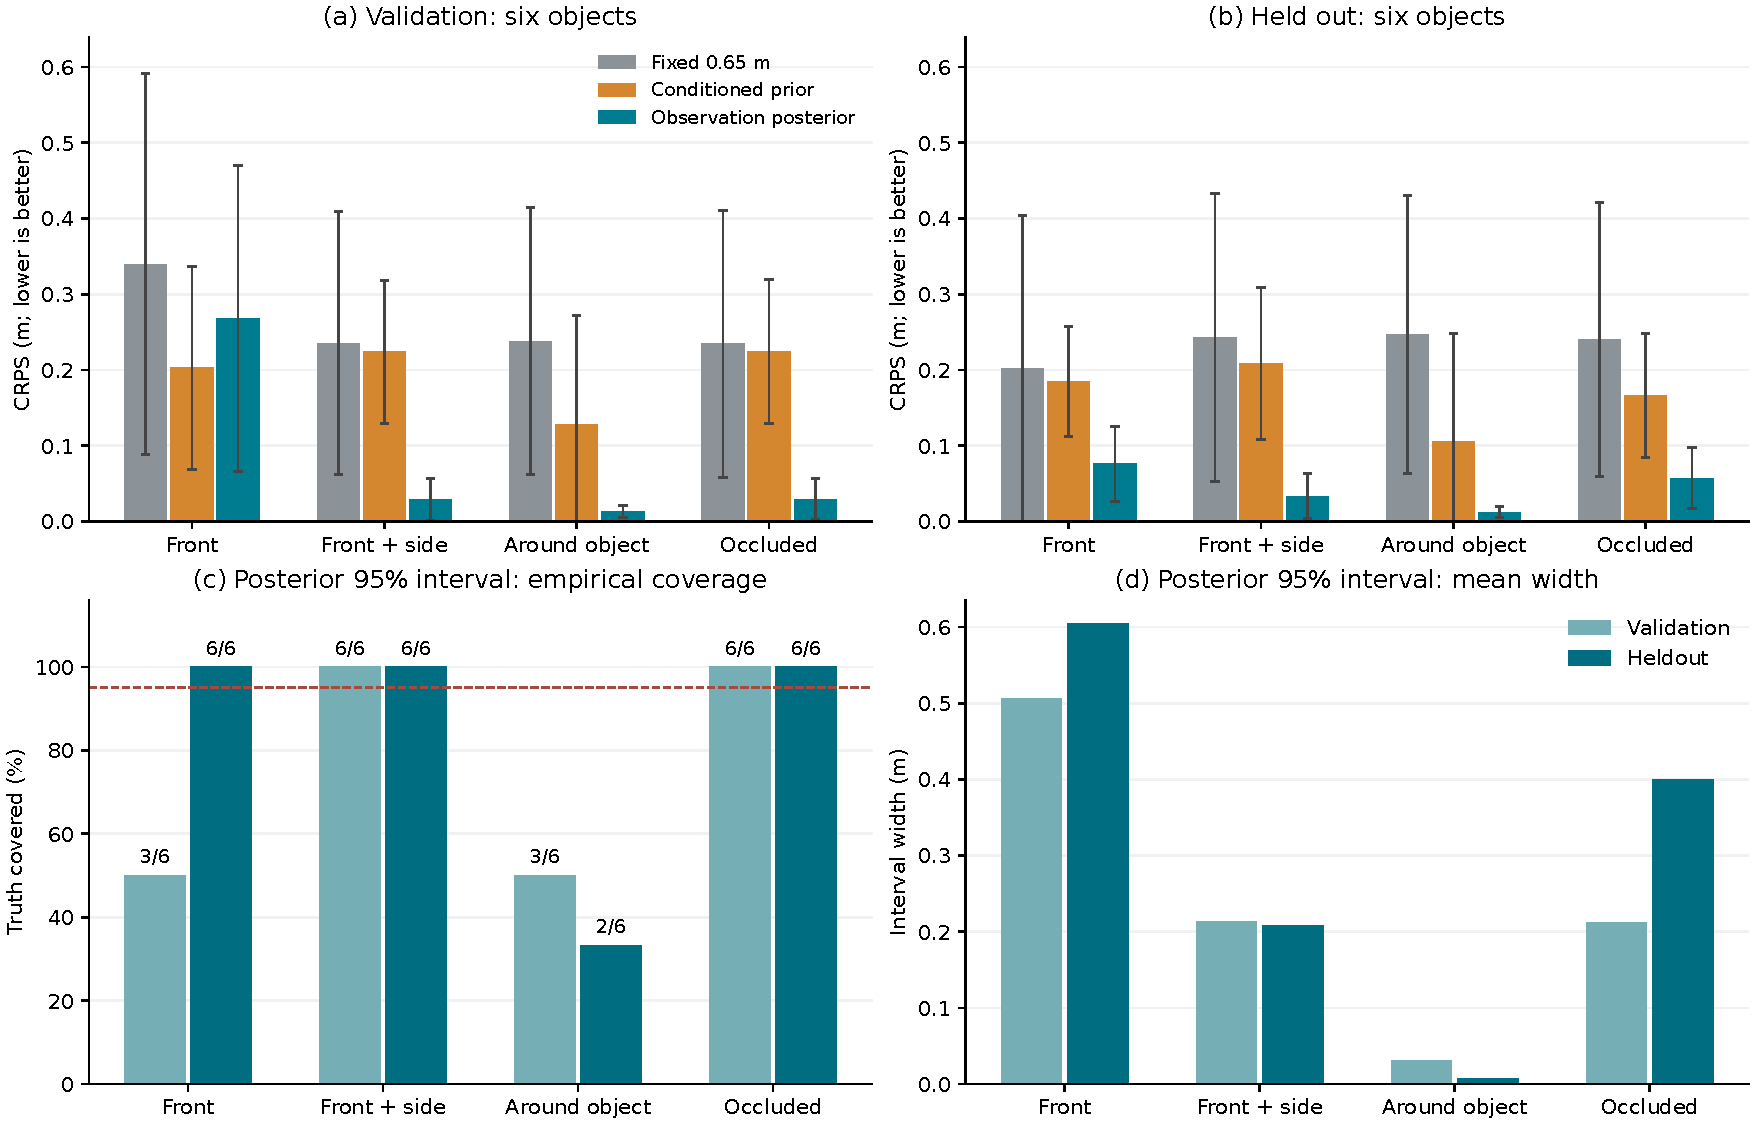
\includegraphics[width=\linewidth]{figures/calibration_distribution.pdf}
 \caption{Independent conditional-depth evaluation. CRPS bars show means
 and sample standard deviations across six objects per split, for every
 observation condition; they are not confidence intervals. One common scale
 was selected using 12 separate training objects. Declared failures use the
 public-prior fallback and remain in the denominator. The lower panels give
 empirical coverage counts and mean widths of nominal 95\% central
 intervals; the dashed line is the requested level, not an achieved
 guarantee. Views and conditions of each object are dependent. The results
 are conditional on orientation, width and part assumptions, exact poses
 and ideal visible instance masks.}
 \label{fig:independent-depth-calibration}
\end{figure}
